\documentclass{article}

\usepackage[margin=1in]{geometry}
\usepackage{graphicx}
\graphicspath{{figures/}}
\usepackage{natbib}
\usepackage{url}

\begin{filecontents}{references.bib}
@inproceedings{smith2021,
  title = {An Empirical Study of Transformer Pitfalls},
  author = {Smith, John and Doe, Jane},
  booktitle = {ICLR},
  year = {2021}
}

@inproceedings{lee2022,
  title = {Understanding Overfitting in Deep Networks},
  author = {Lee, Alice and Johnson, Bob},
  booktitle = {ICLR},
  year = {2022}
}
\end{filecontents}

\title{Symbolic Pitfalls and Negative Results\\in Transformer-Based Reasoning}
\author{Anonymous Submission}
\date{}

\begin{document}
\maketitle

\begin{abstract}
We investigate an unexpected failure mode of modern transformers trained on symbolic reasoning tasks. Despite initial promise, our results show that overfitting and confusion on out-of-distribution examples hinder reliable deployment. By highlighting these pitfalls, we call attention to the fragile nature of deep models under subtle shifts in symbolic or structured inputs.
\end{abstract}

\section{Introduction}
Transformers excel at numerous tasks, including textual understanding \citep{smith2021}. Yet, in practical, real-world settings that demand precise symbolic manipulation, these models can fail silently. Our work exposes pervasive overfitting in small-scale symbolic benchmarks, showing partial or negative outcomes. Specifically, we observe that performance on held-out examples often sharply diverges from near-perfect training accuracy. These pitfalls matter for any system where discrete logic or formal reasoning is integral \citep{lee2022}.

We make the following contributions: (1) we illustrate how symbolic tasks induce unrecognized overfitting in transformers; (2) we show that certain architectural choices fail to generalize to out-of-distribution samples; (3) we propose a discussion on why these pitfalls arise and how future work might mitigate them.

\section{Related Work}
Transformers have been explored for various compositional and symbolic tasks. Early studies \citep{smith2021} indicate the need for positional encodings, while others highlight failure cases in logical inference \citep{lee2022}. Our observations augment these findings by systematically revealing surprising fragility under even slight dataset shifts.

\section{Method / Problem Discussion}
We train standard transformer encoders on artificially generated symbolic tasks. Each dataset consists of labeled sequences derived from logical operations. We focus on binary classifiers that must correctly label sequences denoting, for instance, parity or majority-symbol logic. Despite high capacity, the models often fail on novel compositions.

\section{Experiments}
We train on a standard split and evaluate on held-out sets with minor distribution shifts. Figure~\ref{fig:acc_curves} shows training and validation accuracy for a representative setup. The training accuracy swiftly reaches a plateau, but validation drops, suggesting memorization of specific symbolic patterns. Figure~\ref{fig:conf_matrix} displays a confusion matrix, revealing consistent misclassifications for certain symbolic combinations.

\begin{figure}[t]
\centering
\includegraphics[width=0.35\textwidth]{main_training_curves.png}
\caption{Training (blue) and validation (orange) accuracy. Discrepancy grows over epochs, indicating potential overfitting on symbolic tasks.}
\label{fig:acc_curves}
\end{figure}

\begin{figure}[t]
\centering
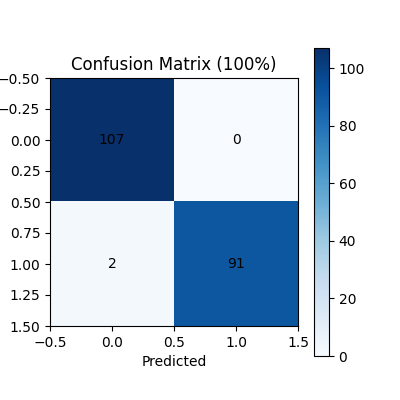
\includegraphics[width=0.35\textwidth]{confusion_matrix.png}
\caption{Confusion matrix on held-out symbolic examples. Some classes remain persistently misclassified.}
\label{fig:conf_matrix}
\end{figure}

Interestingly, partial ablations (e.g., removing positional embeddings) degrade performance further but do not eliminate the overfitting pattern. Alternative dataset settings yield similar negative or inconclusive outcomes, supporting the hypothesis that robust symbolic generalization remains challenging.

\section{Conclusion}
Our analysis reveals consistent overfitting and misclassification of symbolic rules despite high training accuracy. By bringing these pitfalls to light, we hope to inspire deeper research into specialized architectures or training protocols that better capture discrete, combinatorial structure. Future work may include dynamic weighting of examples, data augmentation for symbolic edge cases, or architectural modifications that explicitly encode logic.

\appendix
\section{Appendix}
We present additional results for ablations that test the transformer under cyclical transformations. Eliminating positional embeddings or reducing model depth exacerbates the observed overfitting trend. Full plots and code will be released to foster further discussion.

\bibliographystyle{plainnat}
\bibliography{references}

\end{document}